\documentclass[11pt,a4paper]{article}
\usepackage[margin=2cm]{geometry}
\usepackage{graphicx}
\usepackage{booktabs}
\usepackage{amsmath}
\usepackage{amssymb}
\usepackage{siunitx}
\usepackage[hidelinks]{hyperref}
\usepackage{caption}
\usepackage{float}
\usepackage{enumitem}
\captionsetup{font=small}
\setlist[itemize]{nosep, leftmargin=1.2em}
\setlength{\parskip}{3pt}

\title{A deterministic emulator of the Veros ACC last-year state}
\author{}
\date{31 October 2026}

\begin{document}
\maketitle

\section*{Summary}
\begin{itemize}
  \item Goal: predict the last-year temperature of the Veros ACC channel directly from the EKE-closure
        coefficients $(c_k, c_\epsilon)$, skipping the 100-year integration.
  \item Method: a small deterministic network maps $z = (\log c_k, \log c_\epsilon)$, standardised, to the leading
        PCA coefficients of the training states; it is an ensemble of 5 initialisations. Hyper-parameters come from
        repeated cross-validation with the one-standard-error rule. A fit takes seconds on a CPU.
  \item Interpolation (scattered points, a band of three rows, the $5\times5$ and $7\times7$ centre blocks,
        leave-one-out): RMSE 0.017--\SI{0.038}{K}.
        \begin{itemize}
          \item The nearest training run gives 0.038--\SI{0.118}{K}.
          \item The best classical emulator, a Gaussian process on one collapsed parameter $s$, gives
                0.019--\SI{0.045}{K}. The network is lower on all five evaluations, by 0.0025--\SI{0.0075}{K}.
                With a Holm correction over the eight main evaluations, the difference is significant on four
                ($p \le 0.044$) but not on the scattered split ($p = 0.074$).
        \end{itemize}
  \item Extrapolation (top row, outer 51, outer 75): 0.049 / 0.067 / \SI{0.114}{K}.
        \begin{itemize}
          \item The GP on $s$ gives 0.079 / 0.074 / \SI{0.125}{K}. The network is significantly better on outer 51
                and outer 75 (Holm $p = 0.013$ and 0.004). On the top row most of the gain is one run, and the
                difference is not significant.
          \item The nearest run gives 0.176 / 0.134 / \SI{0.159}{K}.
          \item The warm corner sets the error: \SI{0.16}{K} one row from the training set, \SI{1.06}{K} three cells
                away.
        \end{itemize}
  \item The margin over the GP on $s$ depends on the selection rule.
        \begin{itemize}
          \item With the configuration of minimum CV error instead of the one-standard-error rule, the network is
                still lower on 7 of the 8 evaluations. It ties on the $7\times7$ block and on outer 75, and only
                leave-one-out stays significant after the Holm correction.
          \item The one-standard-error rule was adopted after a first review had seen test errors, so its margins
                are not a blind test.
          \item Against the GP on $z$, the RBF and the nearest run, the network is lower under both rules.
        \end{itemize}
  \item Robustness: four initialisation sets move a split's mean by 0.0004--\SI{0.0010}{K}, and by
        \SI{0.0028}{K} on the top row. Among the configurations that cross-validation cannot tell apart, the test
        error spans up to \SI{0.03}{K}.
  \item Reproducibility: with one BLAS thread, a refit reproduces every number bit for bit. With several
        threads, a split's mean moves by up to \SI{0.0003}{K}.
  \item With four training runs the hyper-parameters cannot be chosen. Depending on them, the network gets
        0.10--\SI{0.19}{K}, against \SI{0.120}{K} for the GP on $s$ (Section~\ref{sec:four}).
\end{itemize}

\section{Data}
\begin{itemize}
  \item 100 Veros ACC runs on a $10\times10$ log-spaced grid, $c_k\in[0.0125,\,0.8]$,
        $c_\epsilon\in[0.0875,\,5.6]$ (ratio $2^{2/3}$); 100 years, 30-day output; interior grid
        $30\times42\times15$ (x, y, z) with a 930-cell ridge.
  \item Target: $y_r \in \mathbb{R}^{17970}$, the mean temperature of the last 12 outputs (360 days) of run $r$
        on the water cells. $S = \SI{35}{psu}$ everywhere, so it is dropped.
  \item The runs still drift, so the averaging window matters. Over the last 20 years, the RMS change from the
        first to the last year is \SI{0.16}{K}, and the last-year mean differs from the 20-year mean by
        \SI{0.08}{K}.
  \item The two parameters act through one combination, $s = \log c_k - 1.08\,\log c_\epsilon$
        (Figure~\ref{fig:data}). Below $s \approx -2$ (48 runs) the domain-mean $T$ stays within
        \SI{0.09}{K}; above, it rises by \SI{1.1}{K}.
\end{itemize}

\begin{figure}[!htb]
\centering
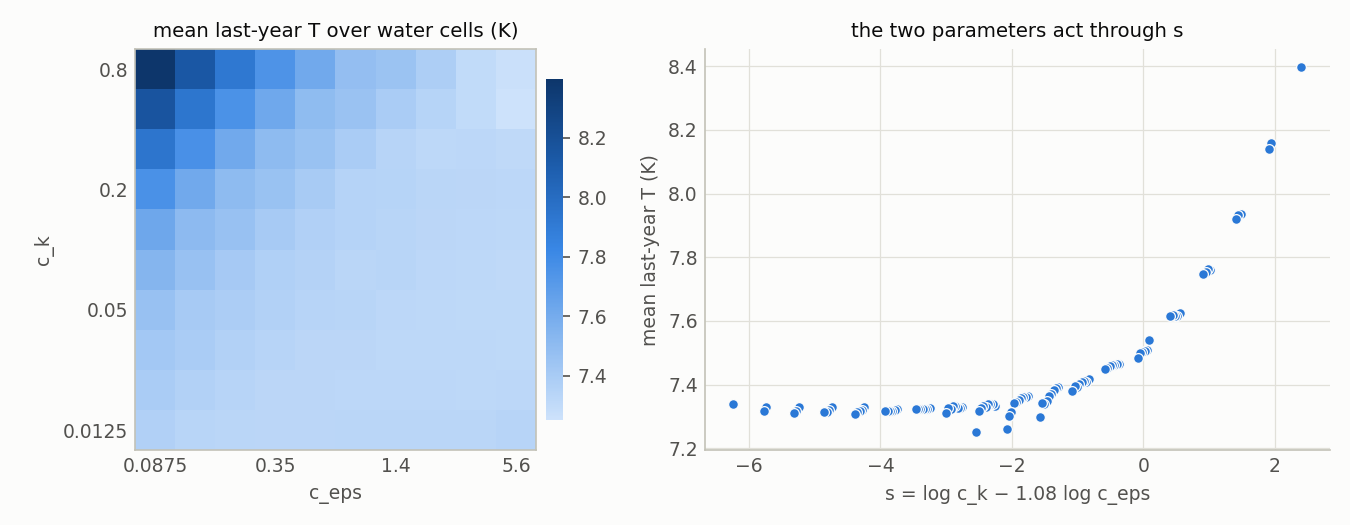
\includegraphics[width=0.9\textwidth]{../results/data.png}
\caption{Mean last-year $T$ over the water cells: over the parameter grid (left) and against $s$ (right), the
direction along which the first PCA coefficient of the states varies linearly.}
\label{fig:data}
\end{figure}

\section{Method}
\label{sec:method}
\begin{itemize}
  \item Input $z$: $(\log c_k, \log c_\epsilon)$ standardised over the design.
  \item Output: a field in the span of the training states,
        \begin{equation}
          \hat y(z) = \mu + \sum_{k=1}^{K} a_k(z)\, v_k, \qquad K = \min(20,\, n - 1),
        \end{equation}
        where $\mu$ and $v_k$ are the mean and the leading principal directions of the $n$ training states.
        So $K = 20$ on every split except the four-run one ($K = 3$).
  \item Network $a(z)$: a multilayer perceptron $2 \to 64 \to 64 \to K$ (scikit-learn, L-BFGS). Its targets are
        $a_k(z_r) = v_k^\top(y_r - \mu)$ divided by $\operatorname{std}(a_1)$, so with orthonormal $v_k$ the data
        term is the physical MSE of the projected field up to a constant. In scikit-learn's normalisation:
        \begin{equation}
          \mathcal{L} = \frac{1}{2nK}\sum_{r=1}^{n} \frac{\lVert a(z_r) - V^\top(y_r - \mu)\rVert^2}{\operatorname{std}(a_1)^2}
          + \frac{\alpha}{2n}\lVert W \rVert^2 .
        \end{equation}
  \item Ensemble: the prediction is the mean of 5 networks that differ only in their initialisation. The whole
        evaluation is repeated with 4 such sets, and reported values average them.
  \item Hyper-parameters: $(\text{activation}, \alpha) \in \{\text{ReLU}, \tanh\} \times
        \{10^{-4}, 10^{-3}, 10^{-2}, 10^{-1}, 1\}$, chosen on the training runs of each split.
        \begin{itemize}
          \item The search is 5-fold cross-validation repeated 3 times. A configuration's CV RMSE is its RMSE
                per training run, averaged over the repeats and then over the runs.
          \item The one-standard-error rule then picks the most regularised configuration whose CV RMSE is within
                one standard error of the best. That standard error is over runs: the standard deviation of the
                best configuration's per-run CV RMSE, over $\sqrt{n}$. It is larger than a standard error over
                folds, so the rule leans towards regularisation.
          \item The choice is ReLU with $\alpha = 10^{-2}$ on every split except outer 75 ($\alpha = 10^{-1}$) and
                four runs ($\alpha = 1$).
          \item The minimum of the same scores is ReLU with $\alpha = 10^{-3}$ or $10^{-4}$, except on outer 75
                ($10^{-2}$) and four runs ($1$).
          \item The rule is not blind to the test sets. It replaced a single 5-fold cross-validation that took the
                minimum, after an independent review had shown that choice to be decided by fold noise, and that
                review had already computed test errors of other configurations. Table~\ref{tab:paired} therefore
                also gives the network chosen by the minimum of the same cross-validation scores.
          \item For leave-one-out the choice is made once, on all 100 runs. Each held-out run therefore takes part
                in it: a mild selection leak, with flat scores.
        \end{itemize}
  \item Fitting on run means rather than on snapshots changes nothing:
        $\sum_t \lVert f(z_r) - x_{r,t}\rVert^2 = n_t \lVert f(z_r) - \bar x_r\rVert^2 + \text{const}$.
  \item Baselines, none tuned by cross-validation (unlike the network):
        \begin{itemize}
          \item the training mean;
          \item the nearest training run in $z$;
          \item thin-plate RBF interpolation of every cell (exact, no smoothing);
          \item a GP per PCA coefficient on $z$ (Mat\'ern 5/2, one length scale per input, white noise up to
                the full variance; hyper-parameters by maximum marginal likelihood);
          \item the same GP on $s = w^\top z$, with $w$ from a linear fit of $a_1$ on $z$.
        \end{itemize}
\end{itemize}

\section{Evaluation}
\begin{itemize}
  \item Eight hold-out splits of the grid, plus leave-one-out over the 100 runs:
        \begin{itemize}
          \item interpolation: 10 scattered interior runs; the rows $c_k$ = 0.126, 0.2, 0.3175; the centre
                $5\times5$ and $7\times7$ blocks;
          \item extrapolation: the top row ($c_k = 0.8$); the 51 or 75 outer runs, training on the centre;
          \item four training runs, one step in from each corner (Section~\ref{sec:four}).
        \end{itemize}
  \item Metric: RMSE over the water cells against the last-year mean, per held-out run, then the mean and
        median over the runs.
  \item Paired comparison with the GP on $s$, on the per-run difference (network RMSE averaged over the 4
        initialisation sets, minus the GP's): its mean, a 95\,\% bootstrap interval, and a Wilcoxon signed-rank
        $p$-value. The $p$-values are also given with a Holm correction over the eight main evaluations (the
        four-run split excluded).
  \item Sensitivity (Table~\ref{tab:sens}): the test RMSE of every configuration on every split, averaged over the
        4 initialisation sets, and the choice of both rules when the cross-validation uses other partitions.
        Neither is used for the selection.
  \item Reproducibility: every fit runs with one BLAS thread.
        \begin{itemize}
          \item With the same library versions (scikit-learn 1.7.2, NumPy 2.2.5, OpenBLAS 0.3.30), a refit
                reproduces every number bit for bit. The sensitivity check refits the chosen configurations in
                other processes and matches every per-run RMSE exactly.
          \item With several threads, L-BFGS stops at a slightly different point. Compared with an earlier run on
                8 threads, a split's mean moved by up to \SI{0.0003}{K}, one initialisation set's mean by up to
                \SI{0.0013}{K}, and a single run by up to \SI{0.008}{K}. Differences of that size are not
                meaningful.
        \end{itemize}
  \item Cost: a fit takes seconds on one core, and a prediction microseconds. On 8 cores the evaluation takes
        46 minutes, mostly the repeated cross-validation and the 100 leave-one-out refits; the sensitivity check
        takes 28 minutes.
\end{itemize}

\begin{table}[H]
\centering\footnotesize\setlength{\tabcolsep}{3pt}
\begin{tabular}{lrrrrrrrrr}
\toprule
split & held out / train & network & range & median & GP on $s$ & GP on $z$ & RBF & nearest & mean state \\
\midrule
scattered & 10 / 90 & \textbf{0.017} & 0.0008 & 0.013 & 0.019 & 0.022 & 0.021 & 0.038 & 0.161 \\
band (three rows) & 30 / 70 & \textbf{0.038} & 0.0010 & 0.033 & 0.045 & 0.051 & 0.057 & 0.118 & 0.204 \\
centre $5\times5$ & 25 / 75 & \textbf{0.025} & 0.0004 & 0.019 & 0.029 & 0.035 & 0.037 & 0.080 & 0.162 \\
centre $7\times7$ & 49 / 51 & \textbf{0.029} & 0.0006 & 0.026 & 0.035 & 0.069 & 0.068 & 0.116 & 0.203 \\
leave-one-out & 100 / 99 & \textbf{0.024} & 0.0004 & 0.017 & 0.028 & 0.032 & 0.034 & 0.085 & 0.221 \\
\midrule
top row & 10 / 90 & \textbf{0.049} & 0.0028 & 0.033 & 0.079 & 0.083 & 0.084 & 0.176 & 0.482 \\
outer 51 & 51 / 49 & \textbf{0.067} & 0.0005 & 0.027 & 0.074 & 0.081 & 0.093 & 0.134 & 0.265 \\
outer 75 & 75 / 25 & \textbf{0.114} & 0.0009 & 0.041 & 0.125 & 0.131 & 0.138 & 0.159 & 0.226 \\
\bottomrule
\end{tabular}

\caption{RMSE (K) of the last-year temperature over the water cells, mean over the held-out runs. Network: mean over
the 4 initialisation sets; range: how much that mean varies across them; median: over the runs. Bold: lowest mean
per split. The four-run split is in Section~\ref{sec:four}.}
\label{tab:main}
\end{table}

\begin{table}[H]
\centering\footnotesize\setlength{\tabcolsep}{3pt}
\begin{tabular}{lrrrrrrrr}
\toprule
 & \multicolumn{3}{c}{one-standard-error rule (reported)} & \multicolumn{5}{c}{minimum CV RMSE} \\
\cmidrule(lr){2-4}\cmidrule(lr){5-9}
split & difference [95\,\% interval] & $p$ & Holm $p$ & choice & network & difference & $p$ & Holm $p$ \\
\midrule
scattered & $-0.0025$ [$-0.0053$, $-0.0005$] & 0.037 & 0.074 & $10^{-3}$ & 0.016 & $-0.0030$ & 0.049 & 0.195 \\
band (three rows) & $-0.0075$ [$-0.0132$, $-0.0020$] & 0.015 & 0.044 & $10^{-3}$ & 0.037 & $-0.0083$ & 0.011 & 0.068 \\
centre $5\times5$ & $-0.0045$ [$-0.0071$, $-0.0019$] & 0.003 & 0.013 & $10^{-4}$ & 0.026 & $-0.0032$ & 0.022 & 0.110 \\
centre $7\times7$ & $-0.0058$ [$-0.0096$, $-0.0021$] & 0.003 & 0.013 & $10^{-3}$ & 0.035 & $+0.0010$ & 0.745 & 1.000 \\
leave-one-out & $-0.0046$ [$-0.0086$, $-0.0015$] & $<0.001$ & $<0.001$ & $10^{-3}$ & 0.023 & $-0.0052$ & $<0.001$ & $<0.001$ \\
\midrule
top row & $-0.0297$ [$-0.0768$, $+0.0001$] & 0.193 & 0.193 & $10^{-4}$ & 0.058 & $-0.0204$ & 1.000 & 1.000 \\
outer 51 & $-0.0076$ [$-0.0123$, $-0.0032$] & 0.002 & 0.013 & $10^{-3}$ & 0.067 & $-0.0072$ & 0.009 & 0.066 \\
outer 75 & $-0.0111$ [$-0.0170$, $-0.0059$] & $<0.001$ & 0.004 & $10^{-2}$ & 0.122 & $-0.0032$ & 0.594 & 1.000 \\
\bottomrule
\end{tabular}

\caption{Network minus GP on $s$, per held-out run (K; negative = network better): the mean difference, its 95\,\%
bootstrap interval, the Wilcoxon signed-rank $p$ and the Holm-corrected $p$ over the eight comparisons. Left: the
network as reported (one-standard-error rule). Right: the network chosen by the minimum CV RMSE instead (ReLU,
with the $\alpha$ given), and its mean RMSE.}
\label{tab:paired}
\end{table}

\begin{table}[H]
\centering\footnotesize\setlength{\tabcolsep}{3pt}
\begin{tabular}{lrrrrrrr}
\toprule
 & \multicolumn{4}{c}{configurations within one standard error} & & \multicolumn{2}{c}{choice, other partitions} \\
\cmidrule(lr){2-5}\cmidrule(lr){7-8}
split & number & test RMSE & below GP on $s$ & rank of the choice & all ten & one SE & minimum \\
\midrule
scattered & 5 & 0.016--0.017 & 5 & 3 & 0.016--0.034 & same & same \\
band (three rows) & 6 & 0.037--0.040 & 6 & 4 & 0.037--0.072 & same & $10^{-2}$ \\
centre $5\times5$ & 5 & 0.025--0.030 & 3 & 1 & 0.025--0.046 & same & $10^{-3}$ \\
centre $7\times7$ & 6 & 0.029--0.045 & 1 & 1 & 0.029--0.060 & same & $10^{-4}$ \\
top row & 5 & 0.049--0.058 & 5 & 1 & 0.049--0.146 & same & $10^{-3}$ \\
outer 51 & 5 & 0.067--0.077 & 3 & 1 & 0.067--0.121 & same & same \\
outer 75 & 6 & 0.114--0.144 & 3 & 1 & 0.114--0.165 & same & same \\
\midrule
four runs & 6 & 0.117--0.187 & 2 & 5 & 0.098--0.187 & same & same \\
\bottomrule
\end{tabular}

\caption{Sensitivity to the configuration. Left: the configurations whose CV RMSE is within one standard error of
the best, the range of their test RMSE (mean over the 4 initialisation sets), how many beat the GP on $s$, and the
rank of the rule's choice among them (1 = lowest test RMSE). All ten: the range over the whole grid. Right: the
choice of each rule when the cross-validation repeats use other partitions (``same'': unchanged).}
\label{tab:sens}
\end{table}

\section{Findings}
\begin{itemize}
  \item \textbf{In interpolation the network has the lowest error of all methods} (Tables~\ref{tab:main}
        and~\ref{tab:paired}, Figure~\ref{fig:splits}).
        \begin{itemize}
          \item Its mean error is 0.25--0.44 times the nearest run's.
          \item Against the GP on $s$ the margin is 0.0025--\SI{0.0075}{K}. After the Holm correction it is
                significant on band, both centre blocks and leave-one-out ($p \le 0.044$). It is not significant
                on the scattered split ($p = 0.074$; 7 of 10 runs better).
        \end{itemize}
  \item \textbf{In extrapolation it is better on outer 51 and outer 75} (Holm $p = 0.013$ and 0.004).
        \begin{itemize}
          \item On the top row the gain (0.049 vs \SI{0.079}{K}) is mostly the warm-corner run (0.16 vs
                \SI{0.37}{K}), and the test is not significant ($p = 0.19$).
          \item Without that run, the network gets 0.037 vs \SI{0.046}{K} and wins 6 of 9.
        \end{itemize}
  \item \textbf{The margin over the GP on $s$ depends on the selection rule} (Table~\ref{tab:paired}, right).
        \begin{itemize}
          \item The minimum CV RMSE picks a weaker regularisation. That network is still lower than the GP on $s$
                on 7 of the 8 evaluations.
          \item It ties on the $7\times7$ block ($+0.0010$\,K, $p = 0.75$) and on outer 75 ($-0.0032$\,K,
                $p = 0.59$).
          \item After the Holm correction only leave-one-out remains significant; band and outer 51 come closest
                ($p = 0.068$ and 0.066).
          \item Its error stays below the GP on $z$, the RBF and the nearest run on every evaluation.
          \item The one-standard-error rule is the more stable choice. With other cross-validation partitions it
                keeps its configuration on all eight splits, while the minimum changes on four
                (Table~\ref{tab:sens}).
          \item But the rule was adopted after the first review had seen test errors of other configurations
                (Section~\ref{sec:method}), so the margins under it are not a blind test.
        \end{itemize}
  \item \textbf{Initialisation matters little, the configuration more} (Tables~\ref{tab:main}
        and~\ref{tab:sens}).
        \begin{itemize}
          \item Four initialisation sets move a split's mean by 0.0004--\SI{0.0010}{K}, and by \SI{0.0028}{K} on
                the top row.
          \item Five or six configurations per split are within one standard error of the best CV score. Their test
                errors span up to \SI{0.03}{K} (outer 75: 0.114--\SI{0.144}{K}).
          \item On scattered, band and the top row, all of them beat the GP on $s$. On the $5\times5$ block,
                outer 51 and outer 75, 3 of them do; on the $7\times7$ block, 1 of 6.
          \item The rule's choice has the lowest test error of the set on five of the seven splits. It ranks third
                of 5 on scattered and fourth of 6 on band.
        \end{itemize}
  \item \textbf{The error sits in the upper \SI{500}{m}} (Figures~\ref{fig:profiles} and~\ref{fig:examples}).
        \begin{itemize}
          \item In interpolation it is 0.014--\SI{0.055}{K} there and 0.003--\SI{0.016}{K} below \SI{1000}{m}.
          \item At the centre of the $7\times7$ block, the predicted anomaly (relative to the training mean) has
                correlation 0.98 with the true one and amplitude 1.05.
          \item This and the other example values are those of Figure~\ref{fig:examples}, which shows the first
                initialisation set.
        \end{itemize}
  \item \textbf{The warm corner} ($c_k = 0.8$, $c_\epsilon = 0.0875$) is the hardest state
        (Figure~\ref{fig:examples}).
        \begin{itemize}
          \item One row from the training set (top row), the network reproduces its warming: correlation 0.99,
                amplitude 0.99, \SI{0.157}{K}.
          \item Three cells away (outer 75), it keeps a weak version of the pattern (correlation 0.62) with a third
                of the amplitude (0.33): a cold bias of \SI{-0.68}{K} and \SI{1.052}{K} RMSE.
          \item Averaged over the four initialisation sets, the network's error there is \SI{1.06}{K}. Every
                method is between 1.06 and \SI{1.45}{K}.
        \end{itemize}
  \item \textbf{Part of the extrapolation error is the basis.} Projecting the held-out truth on the training
        principal directions already leaves 0.010--\SI{0.017}{K} in interpolation and 0.031--\SI{0.079}{K} in
        extrapolation. The outer-75 value (\SI{0.079}{K} of the network's \SI{0.114}{K}) is mostly the corner
        run, where the floor is \SI{0.85}{K}.
  \item \textbf{The spread over initialisations is not an uncertainty.} It is 0.003--\SI{0.009}{K} in
        interpolation and 0.008--\SI{0.011}{K} in extrapolation, while the error grows from 0.017 to
        \SI{0.114}{K}.
  \item The comparison is between a 5-member ensemble and single baselines, and only the network's
        hyper-parameters are tuned by cross-validation.
\end{itemize}

\section{A failure case: four training runs}
\label{sec:four}
\begin{itemize}
  \item Training on $c_k \in \{0.0198, 0.504\} \times c_\epsilon \in \{0.139, 3.53\}$ leaves 96 runs to predict,
        with $K = 3$ principal directions (2 inside the cross-validation folds).
  \item Cross-validation cannot choose here.
        \begin{itemize}
          \item With four runs the 5-fold split is leave-one-out, so the three repeats are identical.
          \item The standard error (\SI{0.15}{K}) covers six configurations.
          \item Both rules pick ReLU with $\alpha = 1$, which also has the minimum CV RMSE.
        \end{itemize}
  \item With that choice the network gets \SI{0.147}{K} (0.134--0.169 over the initialisation sets). The GP on
        $s$ gets \SI{0.120}{K}, the RBF \SI{0.146}{K}, the nearest run \SI{0.181}{K}.
  \item Over the ten configurations the network ranges from 0.10 to \SI{0.19}{K} (Table~\ref{tab:sens}). Among
        the six within one standard error, the choice ranks fifth. The outcome is set by a choice that four runs
        cannot inform.
  \item Regimes:
        \begin{itemize}
          \item where the state saturates ($s < -2$, 46 runs), the medians are 0.040 (nearest run), 0.058
                (network) and \SI{0.061}{K} (GP on $s$);
          \item on the warm side (50 runs) they are 0.197 (network), 0.172 (GP on $s$) and \SI{0.223}{K}
                (nearest run).
        \end{itemize}
  \item With $\alpha = 1$ the network is too flat (Figure~\ref{fig:examples}, rows 2 and 5; first
        initialisation set).
        \begin{itemize}
          \item At the centre run its anomaly has the right pattern (correlation 0.98) with 45\,\% of the
                amplitude: \SI{0.114}{K} (\SI{0.124}{K} over the four sets), against \SI{0.036}{K} for the GP on
                $s$.
          \item At the corner: correlation 0.86, amplitude 0.40, \SI{0.801}{K} (\SI{0.831}{K} over the four
                sets).
        \end{itemize}
\end{itemize}

\section{Next steps}
\begin{itemize}
  \item Inputs $(s, s_\perp)$ instead of $(\log c_k, \log c_\epsilon)$, to build in the collapse that makes the
        GP on $s$ strong with few runs.
  \item For extrapolation, either a decoder not restricted to the span of the training states, or more runs
        near the warm corner.
  \item An uncertainty from resampling the training runs rather than the initialisations.
  \item Tune the baselines by cross-validation as well (RBF smoothing, GP noise and mean function), for an even
        comparison.
  \item Fix the selection rule, or $\alpha$ itself, in advance, and test it on new runs or new splits. Here the
        rule was revised after test errors had been seen, and with very few runs cross-validation cannot choose
        at all.
\end{itemize}

\begin{figure}[!htb]
\centering
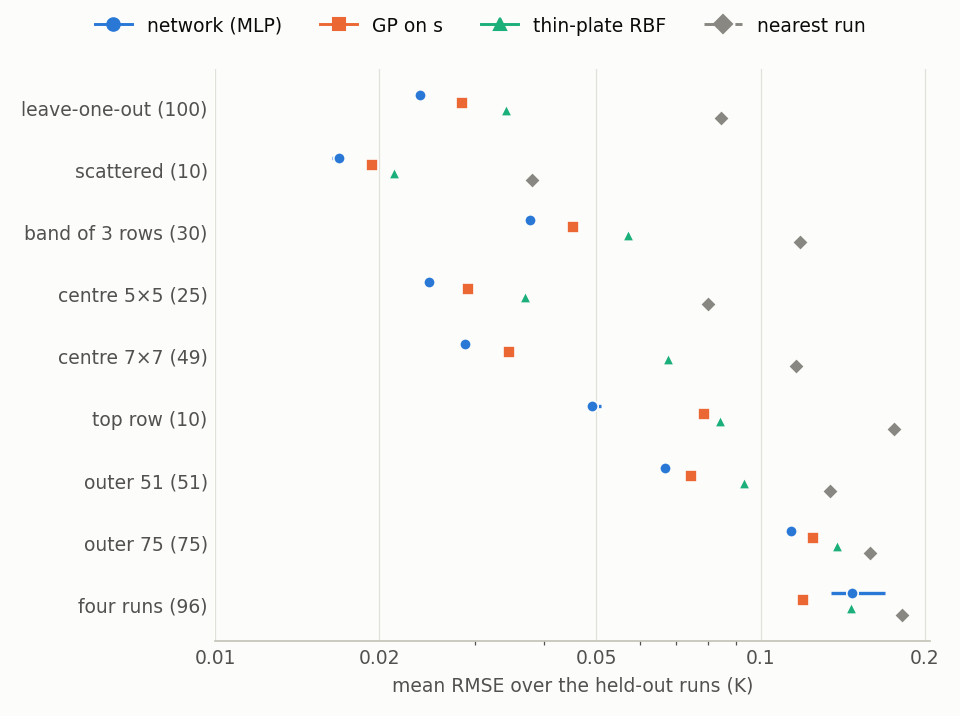
\includegraphics[width=0.72\textwidth]{../results/splits.png}
\caption{Mean RMSE over the held-out runs per split (log scale) for the network and three baselines: the GP on
$s$, the thin-plate RBF and the nearest run. Held-out run counts are in brackets. Network: mean over 4
initialisation sets; the bar is their range.}
\label{fig:splits}
\end{figure}

\begin{figure}[!htb]
\centering
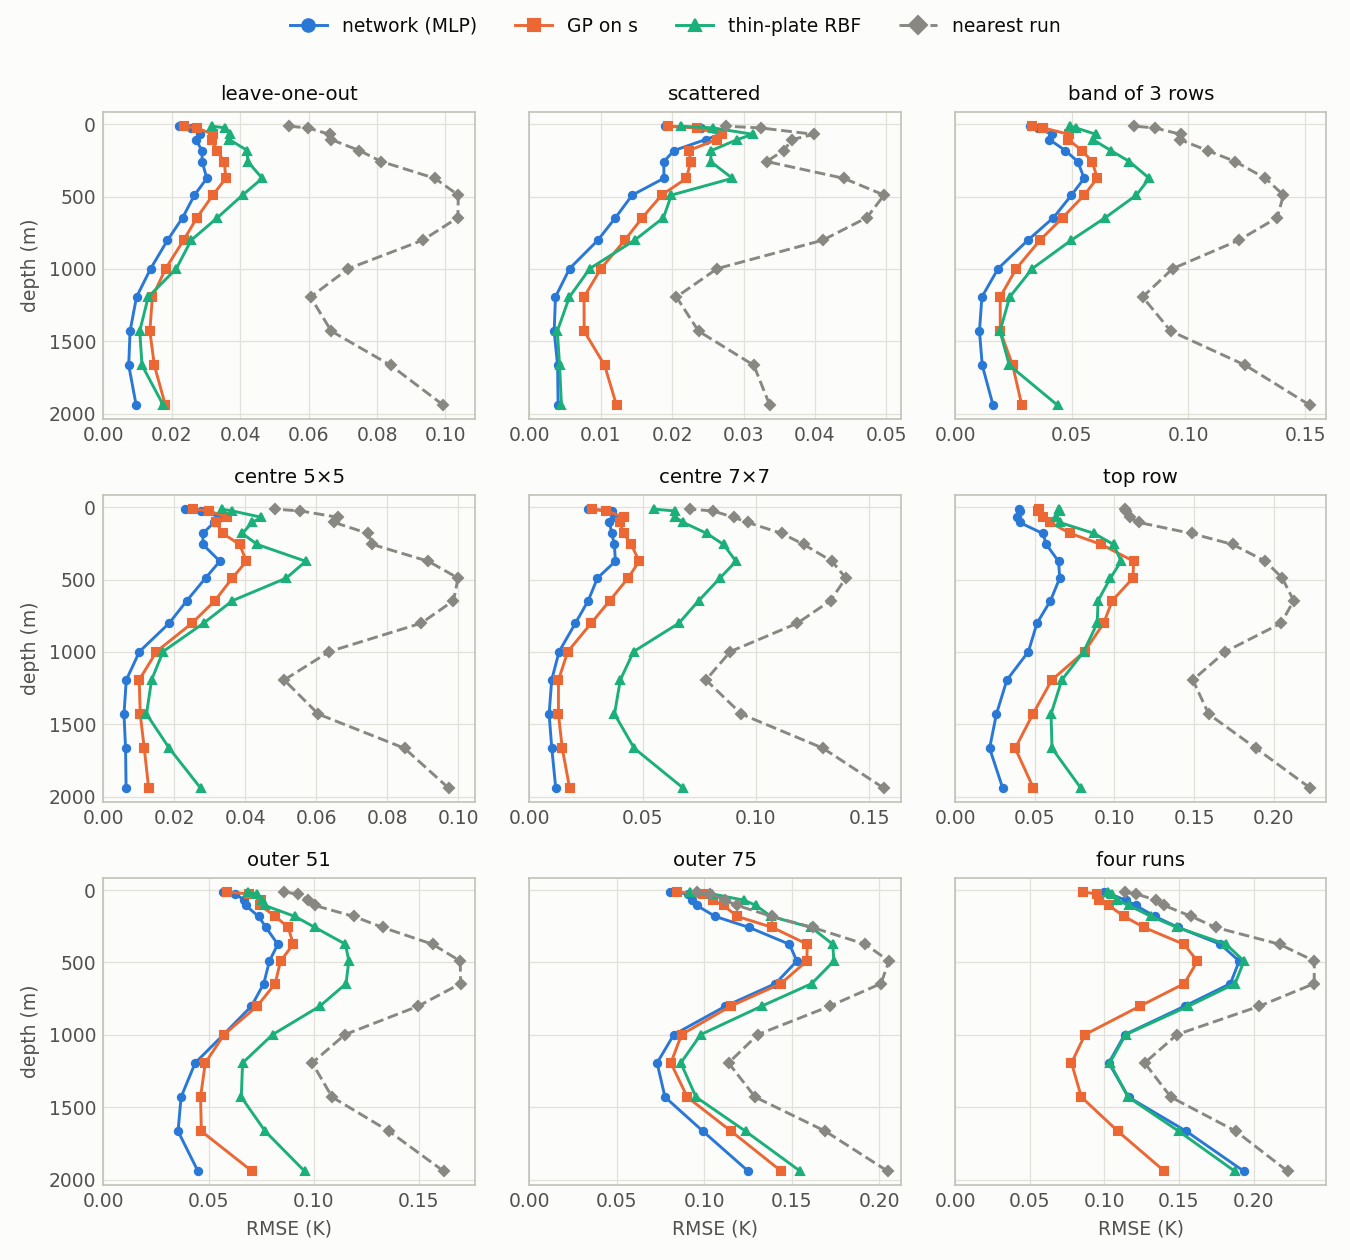
\includegraphics[width=\textwidth]{../results/profiles.png}
\caption{RMSE by depth, mean over the held-out runs of each split (network: averaged over the initialisation
sets).}
\label{fig:profiles}
\end{figure}

\begin{figure}[!htb]
\centering
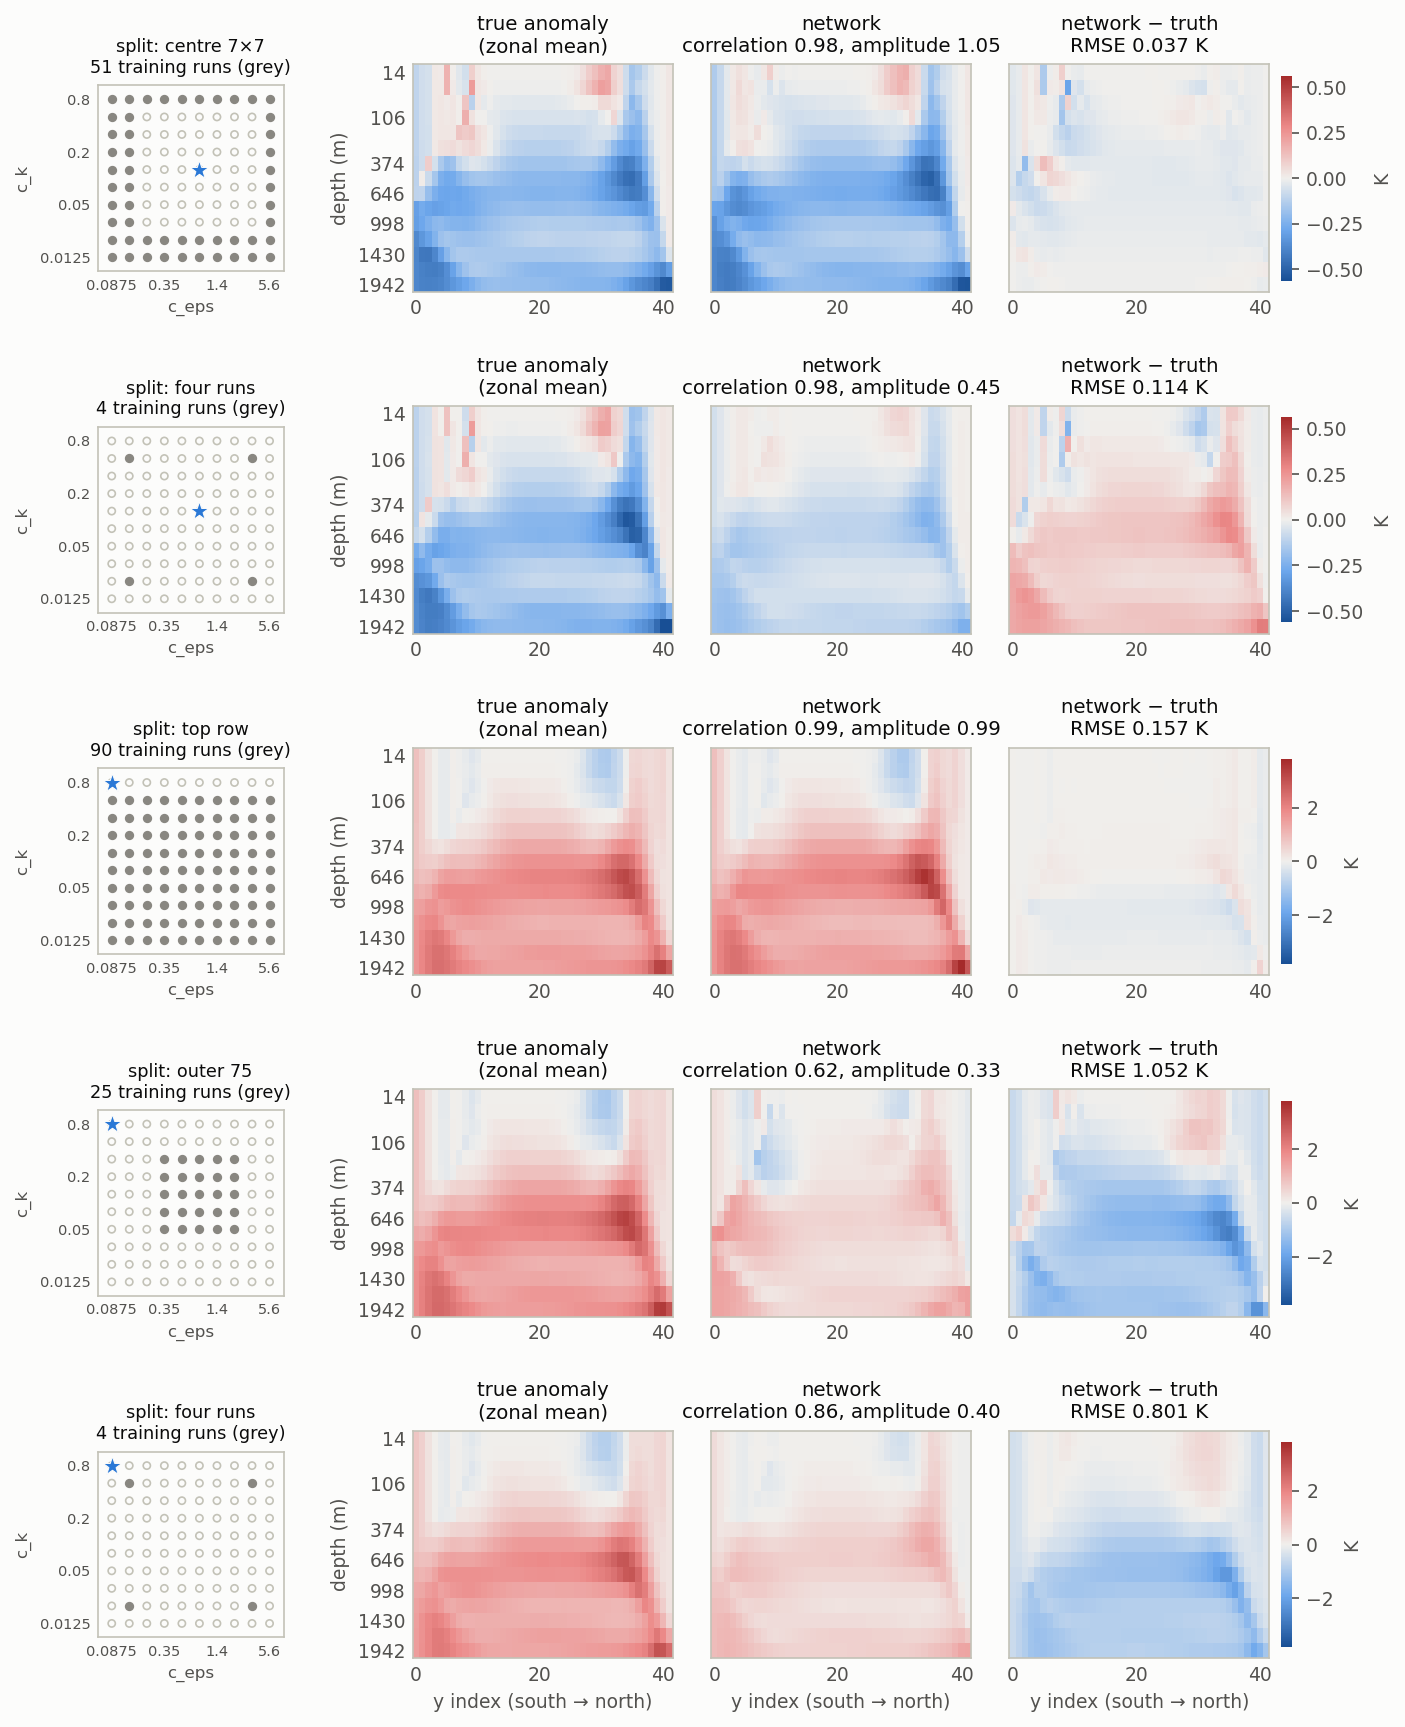
\includegraphics[width=0.93\textwidth]{../results/examples.png}
\caption{Zonal-mean sections of the last-year anomaly, relative to the mean of the split's training runs (what the
network has to add to it): truth, network (first initialisation set) and their difference. Each run has one
colour scale, and levels are drawn with equal height. Left: the split (grey: training runs; open circles: held
out; star: the run shown).
Rows 1--2: the centre run of the $7\times7$ block, held out with the block (51 training runs) and in the
four-run split.
Rows 3--5: the warm-corner run, held out with the top row (90 training runs), with the outer 75 (25) and in the
four-run split (4).
Correlation and amplitude (the regression slope of the predicted on the true anomaly) are over all water
cells.}
\label{fig:examples}
\end{figure}

\end{document}
